\documentclass[a4paper, twocolumn, superscriptaddress,prl]{revtex4}  %% REVTeX 4.0
\usepackage{graphicx}
\usepackage{amsmath,amssymb,braket}

\begin{document}
\title{Quantum enhanced fluorescence microscopy with a single photon avalanche diode array}
\author{Clayton Seitz and Jing Liu}
\affiliation{Department of Physics, Indiana University, Indianapolis}

\begin{abstract}
Localization microscopy uses precise localization of isolated fluorescent emitters to produce super-resolved images. The number of fluorescent emitters is a critical piece of information during localization, which cannot be reliably estimated with conventional microscopies. Photon statistics can potentially provide the necessary physical information for localization in non-sparse scenes by yielding estimates of the number active fluorescent emitters. This work introduces an imaging method for accurately counting active fluorescent emitters, while performing standard intensity-based localization using a single photon avalanche diode (SPAD) array. SPAD cameras, with their high temporal resolution and single photon sensitivity, offer significant advantages relative to standard camera technologies while maintaining the relative simplicity of widefield imaging. Integrating photon statistics with conventional single molecule localization techniques may enhance bioimaging capabilities, building on conventional super-resolution imaging modalities.
\end{abstract}

\maketitle 

\subsection{Introduction}

Far-field optical microscopy is fundamentally limited by diffraction, with the maximum attainable resolution being limited to approximately half the wavelength of light. Several schemes to beat the diffraction limit have been developed in recent years. Many of these schemes utilize the concept of precise localization of isolated fluorescent emitters which blink over a time series of frames. An inherent problem with such methods is the requirement that fluorescent emitters be isolated, slowing down the acquisition of super-resolved images. To address this, gathering additional information on the number of active emitters by computing photon correlation statistics can potentially enable localization in non-sparse scenes \citep{Ta2010}. 

Molecular counting with photon statistics has a fairly simple motivation: coincidence of photons at multiple detector elements during high speed imaging provides evidence for the number of emitters present in the imaged region. Combining the ideas of conventional super-resolution approaches, with photon statistics may prove to be a powerful set of methods for bioimaging. Indeed, single photon arrays technologies, such as SPAD cameras, achieve orders of magnitude higher temporal resolutions than standard CMOS cameras, single photon sensitivity, and theoretically zero readout noise. (Forbes 2019). Furthermore, the reduced readout noise and large fill-factor of the SPAD array suggests its use for single molecule localization with reduced localization uncertainty. Localization uncertainty, typically the RMSE of a maximum likelihood or similar statistical estimator, is bounded from below by the inverse of the Fisher information matrix, known as the Cramer-Rao lower bound (Chao 2016). Managing the increase in localization uncertainty at high labeling density remains a major bottleneck to SMLM. For example, static uncertainty due to molecular crowding can be partially amelioriated by using pairwise or higher-order temporal correlations within a pixel neighborhood \citep{Dertinger2009}. However, the number of fluorescent active emitters in a region of interest remains critical prerequisite information in single molecule localization.

In this study, we present a method for widefield single photon counting in order to rigorously count fluorophores in the sample and subsequently constrain single molecule localization. We investigate the theoretical properties of the zero-lag second-order coherence function $g^{(2)}(0)$ for widefield photon counting and its spatial properties. Using Bayesian analysis, we derive a posterior distribution on the number of active fluorescent emitters in a region of interest. We then combined this with single molecule localization algorithms and demonstrate resolution of multiple emitters using a multi-emitter fitting algorithm and report localization errors with respect to the Cramer-Rao bound.

\subsection{Basic Scheme}

\begin{figure*}
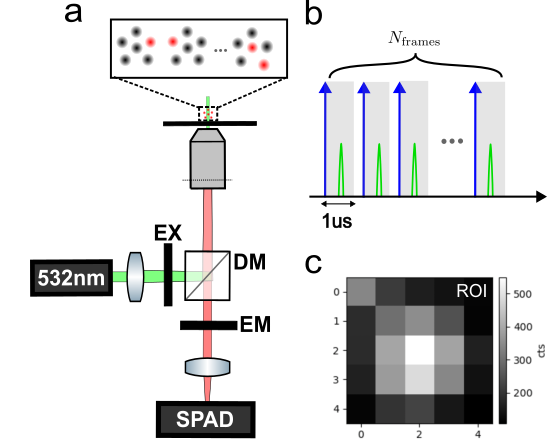
\includegraphics[width=14cm]{Figure-0.png}
\caption{Single photon counting with a SPAD array (a) Conventional widefield microscopy with integrated SPAD array (b) Single photon imaging scheme using 1us exposures containing a picosecond laser pulse (c) Sum of photon counts over a 5x5 region of interest (ROI), taken with $N_{\mathrm{frames}}=5\times 10^{5}$}
\end{figure*}    

We consider a simplified description of widefield photon counting for a a single photon source in the object plane labeled by a continuous-valued coordinate $\theta=(x_0,y_0)$. The spatial profile $O$ of the field in image space is presumed to have a Gaussian shape \citep{Zhang2007}.

\begin{equation}
O(x,y) = \frac{1}{2\pi\sigma^{2}}e^{-\frac{(x-x_{0})^2+(y-y_{0})^2}{2\sigma^2}}
\end{equation}

Therefore the field operator in object space is $\hat{E} \propto \hat{a}$ and in image space $\hat{E} \propto O(x,y)\hat{a}$. Since our SPAD detectors at the image plane must be discrete, the total field at a detector element $n$ centered in image space at $s_k=(u_k,v_k)$ is then given by integrating over pixels of width $\delta$. Moreover, the Gaussian $O$ is presumed to be isotropic and therefore we have $\hat{E}(s_k) \propto \Gamma_{x}(u_k,x_{0})\Gamma_{y}(v_k,y_0)$. For example,

\begin{align*}
\Gamma_{x}(u_k,x_{0}) &= \\ \frac{1}{\sqrt{2}}\left(\mathrm{erf}\left(\frac{u_k+\frac{1}{2}-x_{0}}{\sqrt{2}\sigma}\right) -\mathrm{erf}\left(\frac{u_k-\frac{1}{2}-x_0}{\sqrt{2}\sigma}\right)\right)
\end{align*}

We now consider the case of pulsed excitation where the interval between pulses much longer than the fluorescence lifetime. Upon excitation of an isolated fluorescent emitter, a photon is detected at a particular detector element $k$ with probability $\zeta\propto \langle \hat{E}^{\dagger}(s_k)\hat{E}(s_k)\rangle = \frac{1}{2}\lambda_{x}^2 \lambda_{y}^2\mathrm{Tr}(\rho a^{\dagger}a)$ where $\rho$ is the density matrix for a two-level system. Similarly, the probability of detection in a region of interest collecting all photons emitted is $\zeta\propto \mathrm{Tr}(\rho a^{\dagger}a)$. Here, we are primarily concerned with the latter quantity, and its application in counting fluorescent emitters.

\begin{figure*}
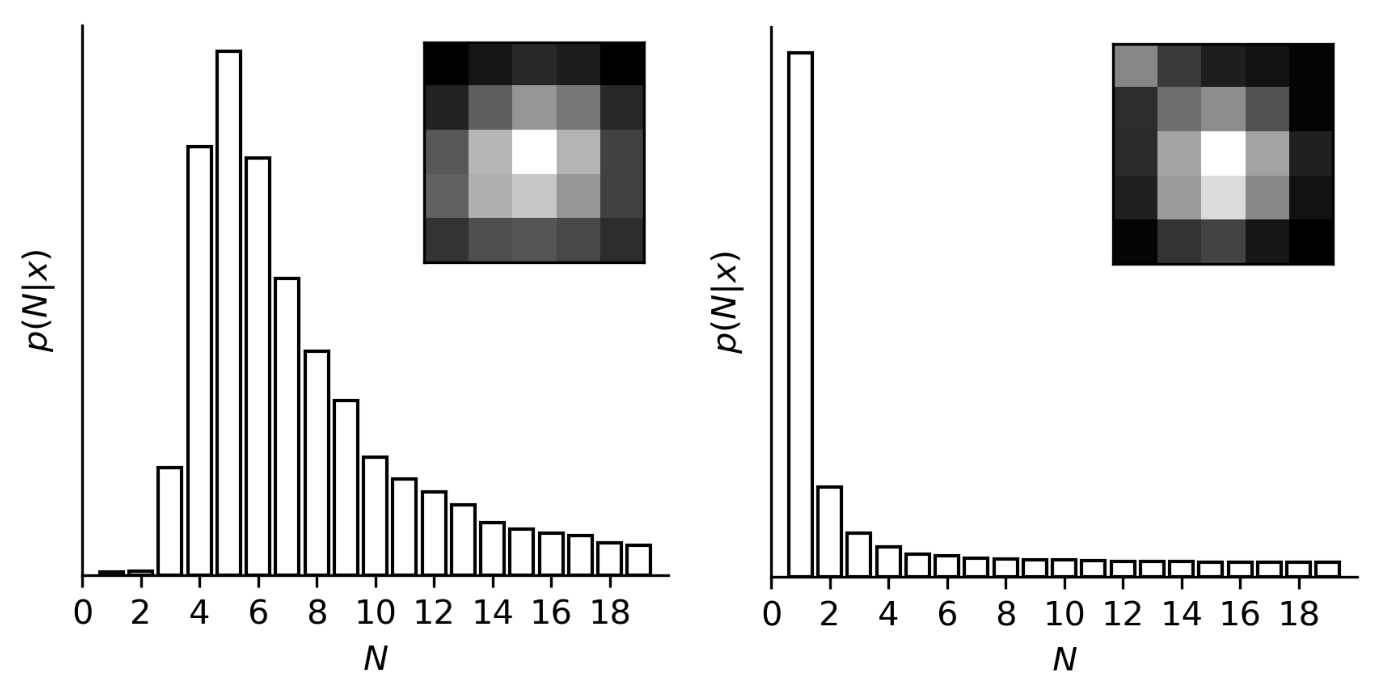
\includegraphics[width=15cm]{Figure-4.png}
\caption{Single molecule localization with a SPAD array. (a) Posteriors on the number of fluorescent emitters and localization of one and two quantum dots (b) Localization uncertainty for simulated data}
\end{figure*}   

Temporarily ignoring the spatial described by (1), we derive a likelihood on the number of fluorophores in a small ROI. Here, we choose a ROI of lateral dimension $d = 5$ pixels. For $N$ fluorophores emitting photons which can be detected within a ROI of the SPAD array, the number of signal photons measured $n_{\mathrm{signal}}$ following a single excitation pulse will have Binomial statistics $n_{\mathrm{signal}} \sim \mathrm{Binom}(N,\zeta)$. Photon pile-up at a single detector element can be safely neglected in this model due to its relatively low likelihood. We then model the background signal within the region of interest as a coherent state, which must follow Poissonian statistics $n_{\mathrm{background}} \sim \mathrm{Poisson}(\lambda)$ for an expected number $\lambda$ of background counts in the ROI per frame. The total number of counts $n=n_{\mathrm{signal}}+n_{\mathrm{background}}$ detected in the region of interest following a single pulse is then distributed by the likelihood

\begin{equation}
p(n=n' \mid N, \zeta) = \sum_{i=0}^{\infty} \binom{N}{i} \zeta^i (1-\zeta)^{N-i} \frac{\lambda^{n'-i}}{(n'-i)!} e^{-\lambda}
\end{equation}

The expression in (2) represents a convolution of Poisson and Binomial probability mass functions. This result is the primary means of inference of the number of active emitters $N$ in a ROI.


\subsection{Results}

 
Fluorophores were excited using a picosecond $532\mathrm{nm}$ pulsed laser triggered at $500\mathrm{kHz}$. Emission light was collected using an oil-immersion 100$\times$ objective with numerical aperture (NA) 1.4 (Nikon). The emission signal was then filtered to exclude the laser line (Semrock) and projected onto the SPAD512 sensor (Pi Imaging Technologies) using a tube lens. A simplified diagram of the complete system is depicted in (Figure 1a). Each acquisition consists of $N=5\times 10^{5}$ frames (500ms), synchronized with each laser pulse, using a $1\mathrm{us}$ exposure per frame (Figure 1b). Using this scheme, we then investigated properties of the zero-lag second order coherence function $g^{(2)}(0)$, using quantum dots coated on a glass coverslip (Figure 1d). The $g^{(2)}(0)$ value is computed over a sliding window ROI to obtain maps of the coherence function over space (Figure 1e). The following empirical estimate of $g^{(2)}(0)$ is used (Israel 2017)

\begin{equation}
g^{(2)}(0) = \frac{G^{(2)}(0)-B}{\langle G^{(2)}(m)\rangle -B}
\end{equation}

where $B = N_{\mathrm{frames}}\lambda\zeta$ is the expected number of background-signal coincidences in the region of interest. The quantity $G^{(2)}(m)$ represents the number of signal-signal coincidences in the region of interest at a lag time $m$.

In order to begin to perform localization in non-sparse ROIs, we write a posterior distribution on the Binomial parameters used in the likelihood (2) using Bayes rule

\begin{equation*}
p(N,\zeta|x) \propto p(x|N,\zeta)p(\zeta)
\end{equation*}

We use a Gaussian prior on $\zeta$ i.e., $p(\zeta) = \mathcal{N}(\mu_{\zeta},\sigma_{\zeta})$. This posterior can be integrated over $\zeta$ to produce a posterior distribution on the fluorophore number $N$ i.e., $p(N=N'|n) \propto \int_{0}^{1} \prod_{j} p(n_{j}|N',\zeta)p(\zeta) d\zeta$ which can be estimated using Monte Carlo methods. The final posterior is then estimated by minibatching the data into batches of $10^3$ frames and averaging the posterior $p(N|n)$ over minibatches. The fluorophore number $N$ within each ROI is then estimated by the maximum aposteriori (MAP) estimate $N^{*}$ given by this distribution.

For localization, we notice that (2) is well approximated by a Poisson distribution for a large frame number, making the localization procedure similar to conventional intensity-based methods \citep{Smith2010}. Denoting the fluorophore coordinates by $\theta$ and vector of total counts in the region of interest $\vec{n}$, we have the following log-likelihood

\begin{align}
\ell(\vec{n}|\theta) &= -\log \prod_{k} \frac{e^{-\left(\mu_{k}\right)}\left(\mu_{k}\right)^{n_{k}}}{n_{k}!}\\
&= \sum_{k}  \log n_{k}! + \mu_{k} - n_{k}\log\left(\mu_{k}\right)
\end{align}

where, in the multi-emitter regime the expected photon count at a pixel is $\mu_{k} = \sum_{m=1}^{N^{*}} \mu_{k,m}$ given $\mu_{k,m}=\zeta N_{\mathrm{frames}}\Gamma_{x}(u_k,x_{0,m})\Gamma_{y}(v_k,y_{0,m}) + \lambda N_{\mathrm{frames}}/d^{2}$. We then use Goodman and Weare's Markov Chain Monte Carlo (MCMC) algorithm to sample from the posterior on fluorophore locations. Fluorophore locations and their uncertainty can then be identified by taking clustering the posterior samples into modes (Figure 2). Our results show that the mean of each identified of posterior cluster is a reasonable estimator of fluorophore locations. 

For an isolated emitter, the Poisson log-likelihood (5) is convenient for computing the Fisher information matrix for $\theta$ and thus the Cramer-Rao lower bound, which bounds the variance of a statistical estimator of $\theta$, from below (Chao 2016). The Fisher information is \citep{Smith2010}

\begin{equation}
I_{ij}(\theta) = \sum_{k}\frac{1}{\mu_{k}}\frac{\partial \mu_{k}}{\partial\theta_{i}}\frac{\partial \mu_{k}}{\partial\theta_{j}}
\end{equation}

The Cramer-Rao bound is then found by $\mathrm{var}(\theta) \geq I^{-1}(\theta)$ and can be used to bound the variance of any statistical estimator of $\theta$ from below. 

\subsection{Discussion}

Many fluorescent emitters exhibit random variations of brightness known as blinking. Blinking increases the observed photon-number fluctuations and could be expected to affect the value of $g^{(2)}(0)$ or the posterior on the number of active fluorescent emitters. However, the signal photon number per frame will follow Binomial statistics even in the presence of blinking, the only consequence of which is an effective reduction of the emission probability. If the effect of censoring photons by blinking and lowering the quantum yield can be accounted for, the technique used here may be compatible with common super-resolution techniques such as stochastic optical reconstruction microscopy (STORM). 

The acquisition times necessary to obtain sufficient photon counts for computing the necessary statistics can potentially be very short. Most fluorophores have relaxation times in the nanosecond range and thus photons can be collected at a rate of at tens of millions of excitation pulses per second. These rates are currently difficult to obtain, however, due to limitations in detector throughput. Current state of the art and commercially available SPAD cameras have a minimum exposure time in the microsecond range. Furthermore, the data volume can quickly become intractable due to the need for several thousands of frames for a millisecond-scale exposure time. This is currently a complication for techniques like STORM and advancements in the automation for data acquisitions are necessary. 

In conclusion, we propose a single molecule imaging technique that allows for simultaneous counting of localization of fluorescent molecules by modeling the quantum properties of fluorescence emission. The technique does not require a nonclassical light source and is designed to supplement standard single molecule localization microscopy techniques. The proposed method can be implemented with a standard widefield fluorescence microscope.



\bibliographystyle{plainnat}
\bibliography{references} 

\end{document}
